\documentclass[12pt]{article}
\textheight = 22cm 
\textwidth = 18cm 
\topmargin = -1cm
\oddsidemargin= -1cm 
\parindent = 0mm 
\usepackage[spanish]{babel}
\usepackage[utf8]{inputenc}
%\usepackage{kmath,kerkis}
%\usepackage[applemac]{inputenc}
\usepackage[T1]{fontenc}
\usepackage[
	hyperref = true,      
  	backend  = bibtex,      
  	sorting  = nyt,       	
  	style  = numeric 	
]{biblatex}
\addbibresource{biblio.bib}
\usepackage{amsmath,amssymb,amsfonts,latexsym}
\usepackage{amsthm}
\usepackage{txfonts}
\usepackage{tikz}
\usepackage{mathtools} 
\usepackage{adjustbox}
\usepackage{wasysym}
\usepackage{graphicx}
\usepackage{physics}
\usepackage{xcolor}
\usepackage{float}
\usepackage{hyperref}
\usepackage{caption}
\usepackage{subcaption}
\usepackage{fancyvrb} % for "\Verb" macro
\VerbatimFootnotes    % enable use of \Verb in footnotes
\usepackage{multicol}
\usepackage{multirow}
\newcommand{\F}{\mathcal{F}} %F bonita
\newcommand{\MSp}[2]{\left(#1, \mathcal{#2}\right)} % Espacio Medible
\newcommand{\EspacioP}[2]{\(\left( #1, \mathcal{#2}, \mathbb{P}\right)} % Espacio de probabilidad 
\newcommand{\salg}[1]{\sigma\left(#1\right)} % sigmaalgebra generada
\newcommand{\letra}[1]{\mathcal{#1}} %letra bonita
\newcommand{\corchete}[1]{\lbrace #1 \rbrace} % corchetes
\newcommand{\R}{\mathbb{R}} % números reales
\newcommand{\N}{\mathbb{N}} % numeros naturales
\newcommand{\Z}{\mathbb{Z}} % números enteros
\newcommand{\Q}{\mathbb{Q}} % numeros racionales
\newcommand{\Esp}[1]{\mathbb{E}\left[#1\right]}
\newcommand{\inverso}[1]{{#1}^{-1}} % inverso de lo que sea
\newcommand{\complem}[1]{{#1}^c} % complemento de un conjunto
\newcommand{\Poten}[1]{\mathcal{P}\left(#1\right)}
\newcommand{\Prob}{\mathbb{P}}
\newcommand{\elem}[2]{\varphi^{-1}_{#1,\dots,#2}}
\newcommand{\paren}[1]{\left(#1\right)}
\newcommand{\sol}{{\textbf{Soluci\'on}}}
\newcommand{\normainf}[1]{\|#1\|_{\infty}}
\newcommand{\card}[1]{{\textbf{card}}\left(#1\right)}
\newcommand{\num}[1]{{\bf{#1}}}
\newcommand{\supp}[1]{\mathbf{supp}\left(#1\right)}
\newcommand{\cl}[1]{\mathbf{cl}\left(#1\right)}
\newcommand{\borel}[1]{\mathcal{B}\paren{#1}}
\newcommand{\indi}[1]{\mathbf{1}_{#1}}
\newcommand*{\QED}[1][$\blacksquare$]{%
\leavevmode\unskip\penalty9999 \hbox{}\nobreak\hfill
    \quad\hbox{#1}%
}
\renewcommand{\epsilon}{\varepsilon}
\renewcommand{\figurename}{Fig.}
\newcommand{\limite}[2]{\lim_{#1\rightarrow #2}}
\newcommand{\E}{\mathbb{E}}
\newtheorem{Teorema}{Teorema}
\newtheorem{Corolario}{Corolario}
\newtheorem{Definición}{Definición}
\newtheorem{Lema}{Lema}

\usepackage{etoolbox,refcount}
\usepackage{multicol}

\newcounter{countitems}
\newcounter{nextitemizecount}
\newcommand{\setupcountitems}{%
  \stepcounter{nextitemizecount}%
  \setcounter{countitems}{0}%
  \preto\item{\stepcounter{countitems}}%
}
\makeatletter
\newcommand{\computecountitems}{%
  \edef\@currentlabel{\number\c@countitems}%
  \label{countitems@\number\numexpr\value{nextitemizecount}-1\relax}%
}
\newcommand{\nextitemizecount}{%
  \getrefnumber{countitems@\number\c@nextitemizecount}%
}
\newcommand{\previtemizecount}{%
  \getrefnumber{countitems@\number\numexpr\value{nextitemizecount}-1\relax}%
}
\makeatother    
\newenvironment{AutoMultiColItemize}{%
\ifnumcomp{\nextitemizecount}{>}{3}{\begin{multicols}{2}}{}%
\setupcountitems\begin{itemize}}%
{\end{itemize}%
\unskip\computecountitems\ifnumcomp{\previtemizecount}{>}{3}{\end{multicols}}{}}


\begin{document}
\title{Análisis de datos de INE y de COVID}
\author{Emilio Villa Cueva\\ Proyecto final del curso de Herramientas Informáticas y Gestión de la Información}
\date{\today}
\maketitle
%\begin{abstract}
 %   Resumen 
%\end{abstract}
\tableofcontents
\newpage
\section{Pronóstico de ocupación de casillas con datos de INE}
\subsection{Problema a resolver}
Con base en los datos recopilados por en INE sobre las listas nominales alrededor del país, disponibles en \cite{ine}, se buscó realizar una estimación de dicha lista nominal para el mes de febrero de 2021. \\
Una vez teniendo una estimación de la lista nominal, el objetivo final del trabajo consistió en estimar el número de casillas necesario por sección dentro del municipio de Guanajuato, bajo la premisa de que por cada 750 mexicanos en la lista nominal se requería una casilla. De manera que:
\begin{equation}
\text{Núm de casillas}=\lceil{\frac{\text{lista nominal}}{750}}\rceil
    \label{eq:1}
\end{equation}
Entonces usando la estimación para febrero de la lista nominal por sección, se podrá calcular el número de casillas requeridas por sección usando la Ecuación \ref{eq:1}. 
\subsection{Procedimiento seguido}
Se trabajó con datos obtenidos la página de internet de \cite{ine}, los datos se encontraban como archivos formato .txt con los valores mensuales de las listas nominales para todo el país. \\
Se trabajo con datos desde marzo de 2019 hasta diciembre de 2020, para poder realizar una estimación lo más exacta posible.
Dentro de dichos datos se separaba la lista en mujeres, hombres, nacionales y extranjeros, también se proporcionaba la lista combinada (mujeres y hombres) nacional. \\
%a partir de aqui modificar para python
Debido a que para los archivos de los diferentes meses en ocasiones se tenían nombres diferentes para la misma variable, lo primero que se hizo fue cambiar el nombre en todos a \textit{LISTA\_N} para la lista nominal, filtrando el estado de Guanajuato y concatenando todos los meses.\\
Posteriormente se agruparon todas las observaciones por municipio para realizar la regresión por municipio, esto también permitió realizar visualizaciones del crecimiento en la lista nominal por municipio como la que se muestra en la figura \ref{fig:1_1}.
\begin{figure}[H]
    \centering
    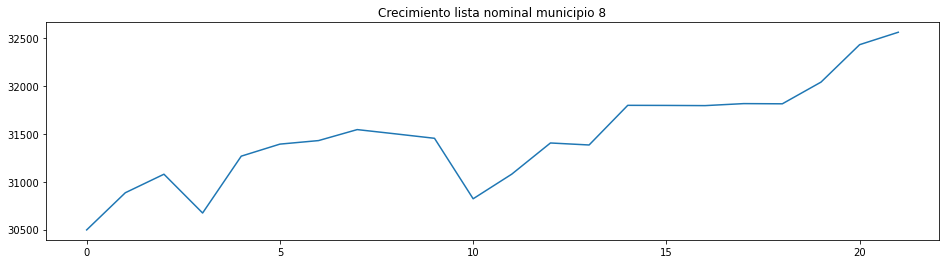
\includegraphics[width=0.7\linewidth]{images/1_1.png}
    \caption{Crecimiento de lista nominal}
    \label{fig:1_1}
\end{figure}
La regresión lineal se realizó usando la implementación del paquete \textit{Scikit-Learn}, usando la función \textit{LinearRegression()}, y usando 22 meses para ajustar los datos (hasta diciembre de 2020), se realizó el pronóstico al  mes de marzo 2021, calculando la tasa de cambio por municipio de la  forma que se muestra en la ecuación \ref{eq:2} y guardándola en un arreglo.
\begin{equation}
\Delta_{nom}^{\text{municipio}}=\frac{LN_{\text{mar2021}}}{LN_{\text{dic2020}}}
    \label{eq:2}
\end{equation}
Teniendo estas tasas de cambio, se procedió a calcular el valor estimado de  la lista nominal por sección, usando los valores de las tasas del municipio al que corresponden, de la forma que se muestra en la figura \ref{eq:3}.
\begin{equation}
LN_\text{mar2021}^{\text{sección x}}=\Delta_{nom}^{\text{municipio}}\times LN_{\text{dic2020}}^{\text{sección x}}
    \label{eq:3}
\end{equation}
De  manera que se pudieron calcular estimaciones para todas las casillas. Finalmente se uso la ecuación \ref{eq:1} para calcular el número necesario de casillas por sección y se sumaron todas las casillas requeridas.
\subsection{Resultados}
Siguiendo este procedimiento, se logró realizar una estimación adecuada para el número de casillas requeridas por sección. Los resultados individuales por casilla se tienen en el archivo, pero en todo el estado se espera que el número total de casillas ronde las \textbf{7620}, que fue el resultado obtenido.\\
Todo se realizó en el \textit{notebook INEforecast.ipynb} adjunto usando \textit{Python 3.8}. Revisar para ver lo que se describe aquí.
\section{Análisis de percepción de afectación de COVID por género alrededor del mundo}
\subsection{Sobre el objetivo del proyecto}
Se trabajó con los datos recopilados por \cite{facebook}, a inicios de la pandemia COVID19 durante julio de 2020 que buscaban dar luz a las dinámicas de género que durante la pandemia se vieron (posiblemente) modificadas alrededor del mundo. \\
A diferencia del reporte anterior, esta vez (además de haber realizado el análisis con Python), se buscó aprovechar más las gráficas de barras para denotar las \textbf{diferencias en la percepción de afectación durante la pandemia} tomando en cuenta las diferentes regiones: Asia del Este, Europa y Asia del Este, Latinoamérica y el Caribe, Medio Oriente y Norte de África, Norteamérica, Sur de Asia y África Sub-Sahariana. Se decidió trabajar con regiones en vez de países ya que se tienen más de 120 países en el conjunto de datos.\\ Este tipo de gráficos (gráficos de barra), aunque sencillos, son capaces de capturar diferencias importantes entre regiones respecto a las afectaciones en diferentes ámbitos, como se verá a continuación.\\
\subsection{Procedimiento seguido}
Primero conviene describir el tipo de datos con los que se trabajó. Consisten en porcentajes de respuestas \textbf{afirmativas} a preguntas específicas realizadas por Facebook a personas en todo el mundo respecto a las afectaciones de la pandemia en diferentes ámbitos, los datos se separan en respuestas de mujeres, de hombres y combinadas. Se tienen las respuestas a más de 80 interrogantes distintas, que buscar dar luz a diferentes aspectos de la vida de la gente alrededor del mundo. En el presente proyecto se decidió trabajar en particular con  8 preguntas de la encuesta que se consideraron de interés:
\begin{itemize}
    \item \textbf{a1\_agree}: De acuerdo con que hombres y mujeres deben de tener las mismas oportunidades
    \item \textbf{c2\_clean}: El encuestado se encarga de la limpieza de la casa
    \item \textbf{c2\_cook}: El encuestado se encarga de cocinar en la casa
    \item \textbf{c3\_agree}: El encuestado está de acuerdo con que el rol más importante de una mujer es cuidar la casa y su familia.
    \item \textbf{c2d\_increase}: Durante la pandemia aumentó el tiempo que se dedica al hogar
    \item \textbf{d5\_agree}: Se ha sentido incómod@ o en riesgo en su propio hogar
    \item \textbf{d7\_money}: Su principal preocupación durante la pandemia es tener dinero sufuiente para subsustir
    \item \textbf{d6\_school}: Se vió imposibilitado de ir a la escuela.
\end{itemize}
Por ejemplo, una observación típica\footnote{Habiendo filtrado ya las variables de interés de la lista.} sería como la que se muestra en la figura \ref{fig:2_1}.
\begin{figure}[H]
    \centering
    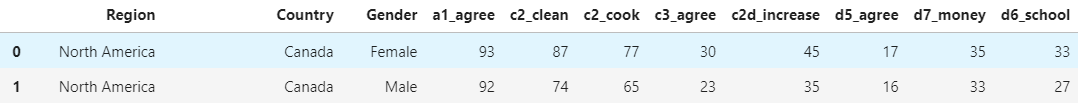
\includegraphics[width=0.9\linewidth]{images/2_1.PNG}
    \caption{Observación típica de los datos}
    \label{fig:2_1}
\end{figure}
Tras haber seleccionado las variables de interés, se procedió a calcular la media por región de cada una de estas variables, generando un \textit{dataframe} para hombres y otro para mujeres, el cual se muestra en el cuadro \ref{table:1}.
% Please add the following required packages to your document preamble:
% \usepackage{graphicx}
\begin{table}[H]
\centering
\resizebox{\textwidth}{!}{%
\begin{tabular}{|l|l|l|l|l|l|l|l|l|l|}
\hline
\textbf{} & Region                                & \textbf{a1\_agree} & \textbf{c2\_clean} & \textbf{c2\_cook} & \textbf{c3\_agree} & \textbf{c2d\_increase} & \textbf{d5\_agree} & \textbf{d7\_money} & \textbf{d6\_school} \\ \hline
1         & \textbf{East Asia \& Pacific}         & 90.416             & 66.1667            & 50.9167           & 51.1667            & 42.583                 & 33.5               & 32.5               & 36.75               \\ \hline
2         & \textbf{Europe and Central Asia}      & 91.846             & 83.0               & 70.795            & 35.538             & 38.564                 & 23.1026            & 35.82              & 30.256              \\ \hline
3         & \textbf{Latin America and Caribbean}  & 91.762             & 80.62              & 62.5714           & 35.095             & 56.143                 & 38.7143            & 54.143             & 44.714              \\ \hline
4         & \textbf{Middle East and North Africa} & 89.706             & 74.0               & 58.7647           & 55.294             & 53.882                 & 43.1176            & 36.529             & 35.471              \\ \hline
5         & \textbf{North America}                & 91.5               & 87.5               & 77.5              & 33.5               & 44.0                   & 15.5               & 37.0               & 34.5                \\ \hline
6         & \textbf{South Asia}                   & 89.7143            & 64.43              & 58.7143           & 62.714             & 53.857                 & 29.714             & 28.428             & 41.571              \\ \hline
7         & \textbf{Sub-Saharan Africa}           & 86.44              & 67.28              & 58.04             & 64.92              & 49.12                  & 50.64              & 36.12              & 51.68               \\ \hline
\end{tabular}%
}
\caption{Dataframe con media de respuestas afirmativas a diferentes variables de interés}
\label{table:1}
\end{table}
De la información de estos \textit{dataframes} es posible generar visualizaciones muy interesantes que sirven para realizar un análisis.
\subsection{Panorama general de afectaciones}
Antes de contrastar entre hombres y mujeres, se tomaron las respuestas de ambos hacia algunas de las preguntas que se consideraron de interés. Las respuestas se ilustran en la figura \ref{fig:21}.
\begin{figure}
     \centering
     \begin{subfigure}[b]{0.45\textwidth}
         \centering
         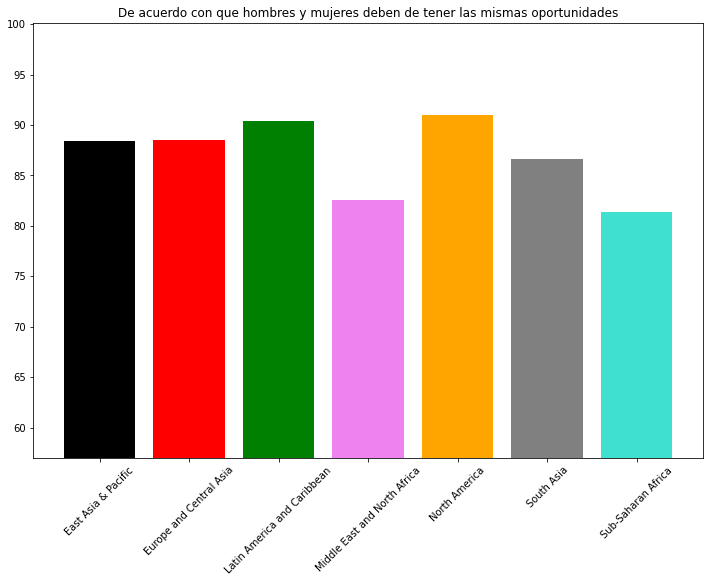
\includegraphics[width=\textwidth]{images/211.png}
         \caption{}
         \label{fig:211}
     \end{subfigure}
     \hfill
     \begin{subfigure}[b]{0.45\textwidth}
         \centering
         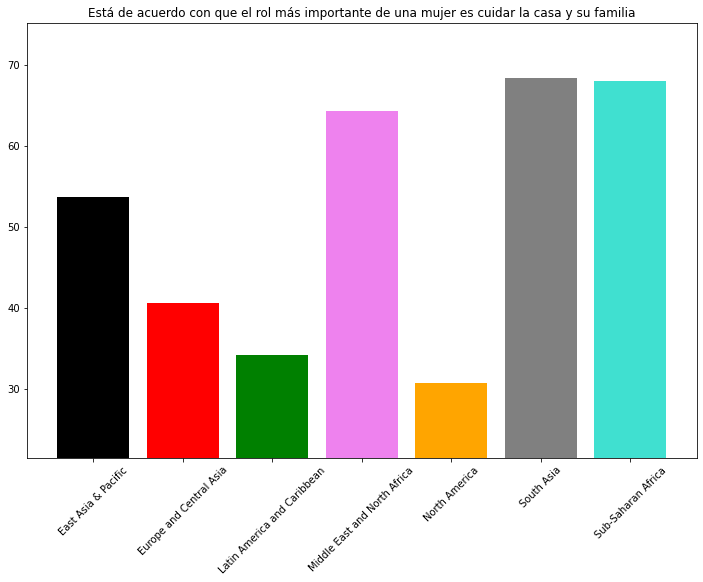
\includegraphics[width=\textwidth]{images/212.png}
         \caption{}
         \label{fig:212}
     \end{subfigure}
     \hfill
     \begin{subfigure}[b]{0.45\textwidth}
         \centering
         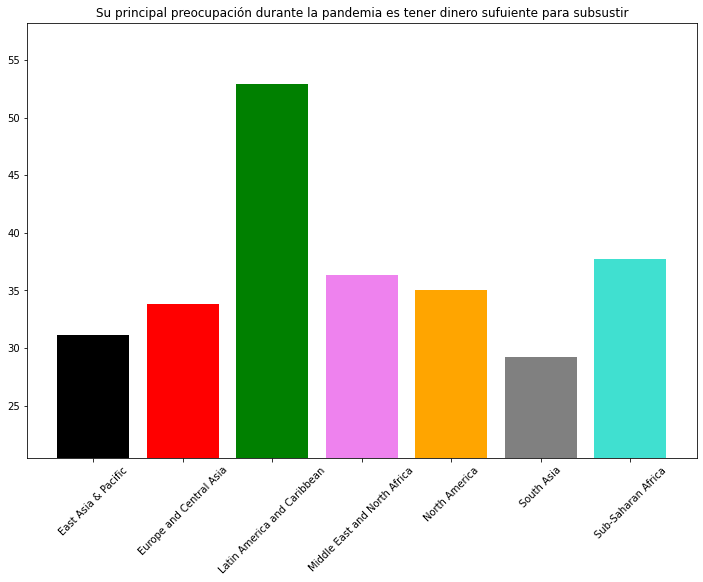
\includegraphics[width=\textwidth]{images/213.png}
         \caption{}
         \label{fig:213}
     \end{subfigure}
     \hfill
     \begin{subfigure}[b]{0.45\textwidth}
         \centering
         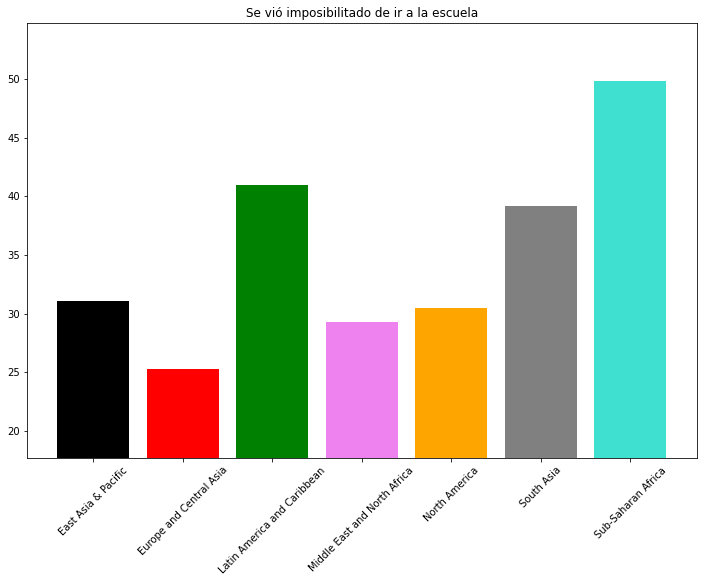
\includegraphics[width=\textwidth]{images/214.png}
         \caption{}
         \label{fig:214}
     \end{subfigure}
        \caption{Afectaciones en diferentes ámbitos}
        \label{fig:21}
\end{figure}
Estar primer parte, más que contrastar diferencias de afectación por género, busca analizar cómo se vieron afectadas diferentes regiones del mundo por efecto de la pandemia, así como las percepciones (tanto de hombres como de mujeres) del rol de  las mujeres en la sociedad.\\
Por ejemplo, se observan regiones donde aún no se considera que la mujer y el hombre deban de tener las mismas oportunidades (figura \ref{fig:211}). Y aún se considera que el rol principal de la mujer es el cuidar de la casa (figura \ref{fig:212}), habiendo regiones como el sur de Asia, África y Medio Oriente donde más de la mitad de la población opina eso.\\
Respecto a la afectación por efecto de la pandemia en un aspecto más general, se puede observar que en los ámbitos económicos (figura \ref{fig:213}) y de educación (figura \ref{fig:214}) América Latina y el sur de África destacan como los más afectados.
\subsection{Contraste entre afectación a hombres y a mujeres}
En esta sección el procedimiento seguido fue que para cada una de las preguntas de interés, y por cada región, se calculó la diferencia entre las respuestas\footnote{Las respuestas afirmativas, es decir, el porcentaje de encuestados que contestó afirmativamente a la pregunta que se le hizo} de las mujeres y de los hombres, como se muestra en la ecuación \ref{eq:21}.
\begin{equation}
\Delta \% = \%_{\text{F}}-\%_{\text{M}}
    \label{eq:21}
\end{equation}
Esto con el interés de mostrar de una manera más clara preguntas donde alguno de los géneros se vio más afectado por región. Los resultados se ilustran entonces en las figuras \ref{fig:22_1} y \ref{fig:22_2}. 
\\De las visualizaciones podemos puntualizar algunas observaciones interesantes. Primero, en la figura \ref{fig:221} notamos que en Medio Oriente, una zona donde existe una brecha grande aún entre los derechos del hombre y de la mujer, la proporción de mujeres que considera que se necesitan derechos iguales es considerablemente mayor que los hombres. De las figuras \ref{fig:222},  \ref{fig:223} y \ref{fig:225}, notamos dos cosas: durante la pandemia fue a mujer quien \textbf{en todo el mundo} se encargo mayoritariamente del hogar (o al menos de la cocina y la limpieza), y al observar la figura \ref{fig:224} notamos que si bien son los hombres quien en la mayoría de las regiones consideran que las tareas del hogar son responsabilidad de la mujer, en América, es mayor la cantidad de mujeres que opinan que las responsabilidades del hogar son de ellas.\\
Un resultado curioso es el de la figura \ref{fig:226}, que hace alusión a si la gente se sintió insegura en su hogar, donde por algún motivo en el sur de Asia fueron en su mayoría los hombres quienes se sintieron inseguros, aunque en el resto del mundo (y probablemente por casos de violencia doméstica que escalaron durante las cuarentenas) fueron las mujeres quienes se sintieron más inseguras. Un resultado similar se obtiene en la figura \ref{fig:227}, donde si bien en la mayoría de las regiones fueron las mujeres quienes se preocuparon más por la economía del hogar, en Asia y África los hombres se encontraban más preocupados. Finalmente, se observa en la figura \ref{fig:228} que fueron las mujeres quienes faltaron más a la escuela por efecto de la pandemia.\\
\begin{figure}
     \centering
     \begin{subfigure}[b]{0.45\textwidth}
         \centering
         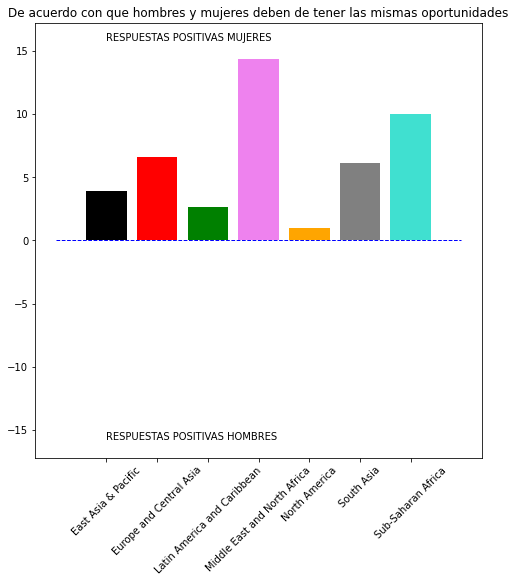
\includegraphics[width=\textwidth]{images/221.png}
         \caption{}
         \label{fig:221}
     \end{subfigure}
     \hfill
     \begin{subfigure}[b]{0.45\textwidth}
         \centering
         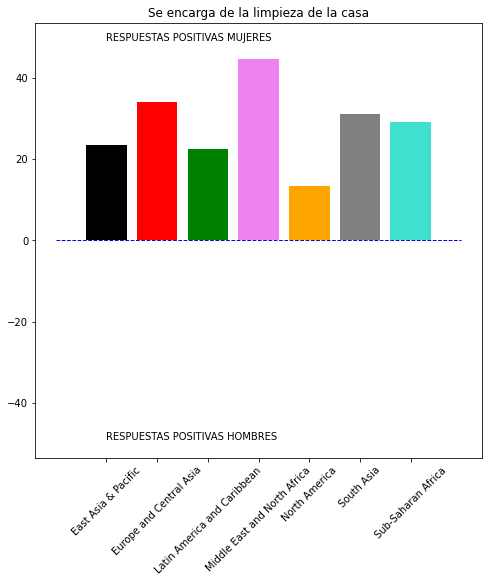
\includegraphics[width=\textwidth]{images/222.png}
         \caption{}
         \label{fig:222}
     \end{subfigure}
     \hfill
     \begin{subfigure}[b]{0.45\textwidth}
         \centering
         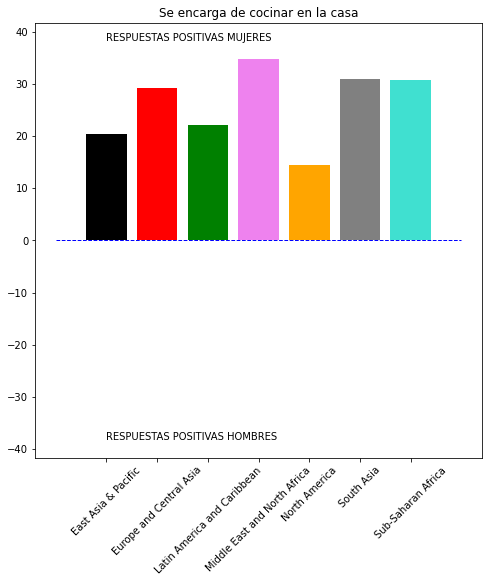
\includegraphics[width=\textwidth]{images/223.png}
         \caption{}
         \label{fig:223}
     \end{subfigure}
     \hfill
     \begin{subfigure}[b]{0.45\textwidth}
         \centering
         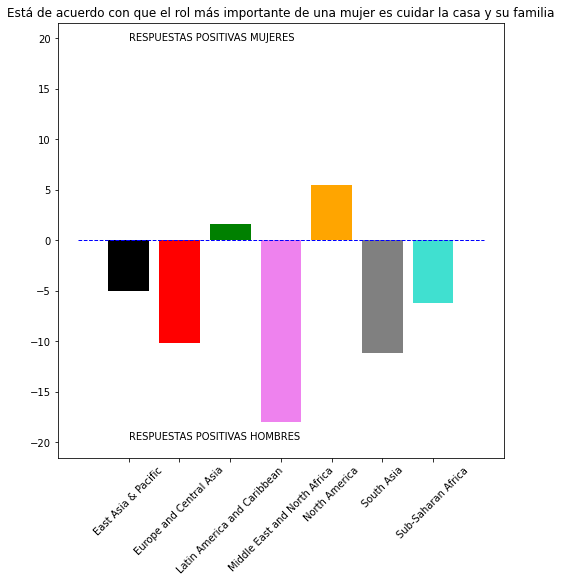
\includegraphics[width=\textwidth]{images/224.png}
         \caption{}
         \label{fig:224}
     \end{subfigure}
        \caption{Afectaciones en diferentes ámbitos}
        \label{fig:22_1}
\end{figure}
\begin{figure}
     \centering
     \begin{subfigure}[b]{0.45\textwidth}
         \centering
         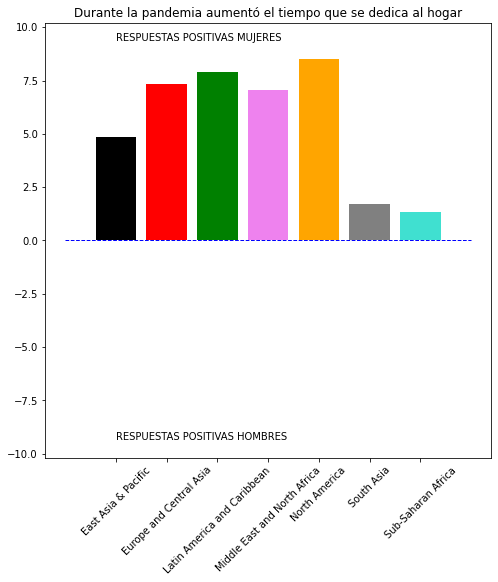
\includegraphics[width=\textwidth]{images/225.png}
         \caption{}
         \label{fig:225}
     \end{subfigure}
     \hfill
     \begin{subfigure}[b]{0.45\textwidth}
         \centering
         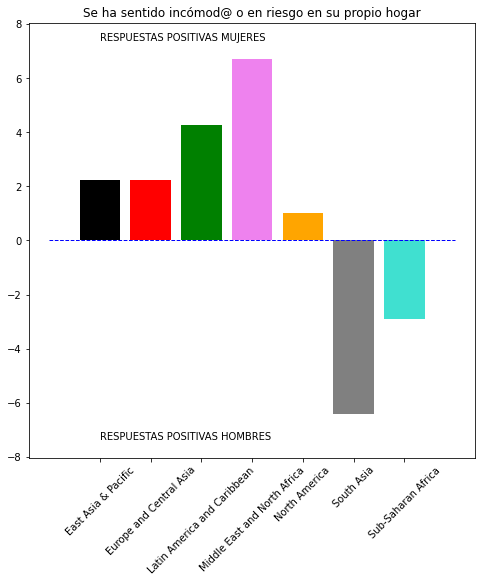
\includegraphics[width=\textwidth]{images/226.png}
         \caption{}
         \label{fig:226}
     \end{subfigure}
     \hfill
     \begin{subfigure}[b]{0.45\textwidth}
         \centering
         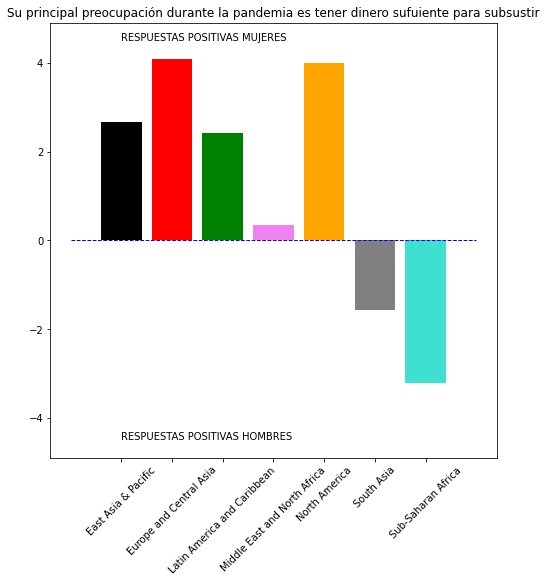
\includegraphics[width=\textwidth]{images/227.png}
         \caption{}
         \label{fig:227}
     \end{subfigure}
     \hfill
     \begin{subfigure}[b]{0.45\textwidth}
         \centering
         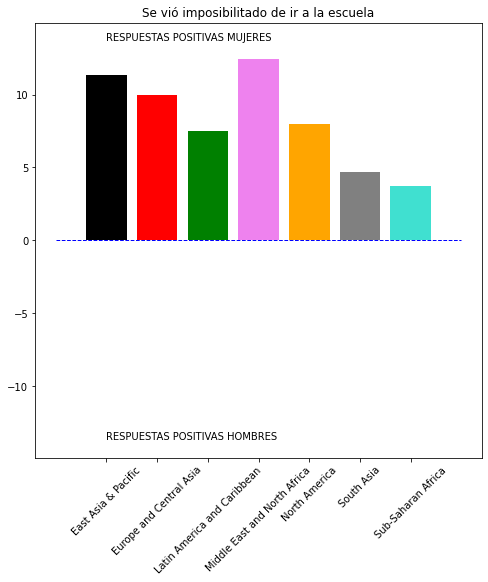
\includegraphics[width=\textwidth]{images/228.png}
         \caption{}
         \label{fig:228}
     \end{subfigure}
        \caption{Afectaciones en diferentes ámbitos}
        \label{fig:22_2}
\end{figure}
\subsection{Sobre el notebook}
Se anexa el notebook \textit{covidAnalysis.ipynb}, donde se realizó todo lo mencionado en ésta segunda sección relativo a los datos de COVID, los datos también se encuentran en \textit{rawData.csv} dentro de la carpeta \textit{data}.

\printbibliography[heading=bibintoc]

\end{document}
